\documentclass{article}
\usepackage{amsmath}
\usepackage{amssymb}
\usepackage{graphicx}
\usepackage[margin=1in]{geometry}
\usepackage{hyperref}
\usepackage{caption}
\usepackage{float}
\graphicspath{{images/}}
\hypersetup{
  colorlinks=true,
  urlcolor=blue,
}
\begin{document}

\title{Game Notes}
\author{Aresh Pourkavoos}
\maketitle

Position within square stored as an odd signed integer in half-pixels,
e.g.
\begin{center}
  \begin{tabular}{|c|c|c|c|}
    \hline
    101 & 011 & 001 & 011 \\ \hline
    -3 & -1 & 1 & 3 \\ \hline
  \end{tabular}
\end{center}
Requires entities to have odd pixel dims to be centered \\
Edge/vertex states are not possible \\
Updating position requires doubling velocity first \\
Store position as $x$ and $y$ seen on screen
or relative to a square's axes? \\
Screen position: 
\begin{itemize}
\item
  Graphics and movement are easier
\item
  Collision would be most convenient by loading the current square rotated
\end{itemize}
Relative position:
\begin{itemize}
\item
  Collision is easier, just check against stored square
\item
  Need to ensure that rendering is done correctly
\end{itemize}
View splitting is decided by determinant sign:
will always give edge to cell further (counter?)clockwise \\
Vertices/edges are on the border between pixels (even position):
do not require a special case
\begin{center}
  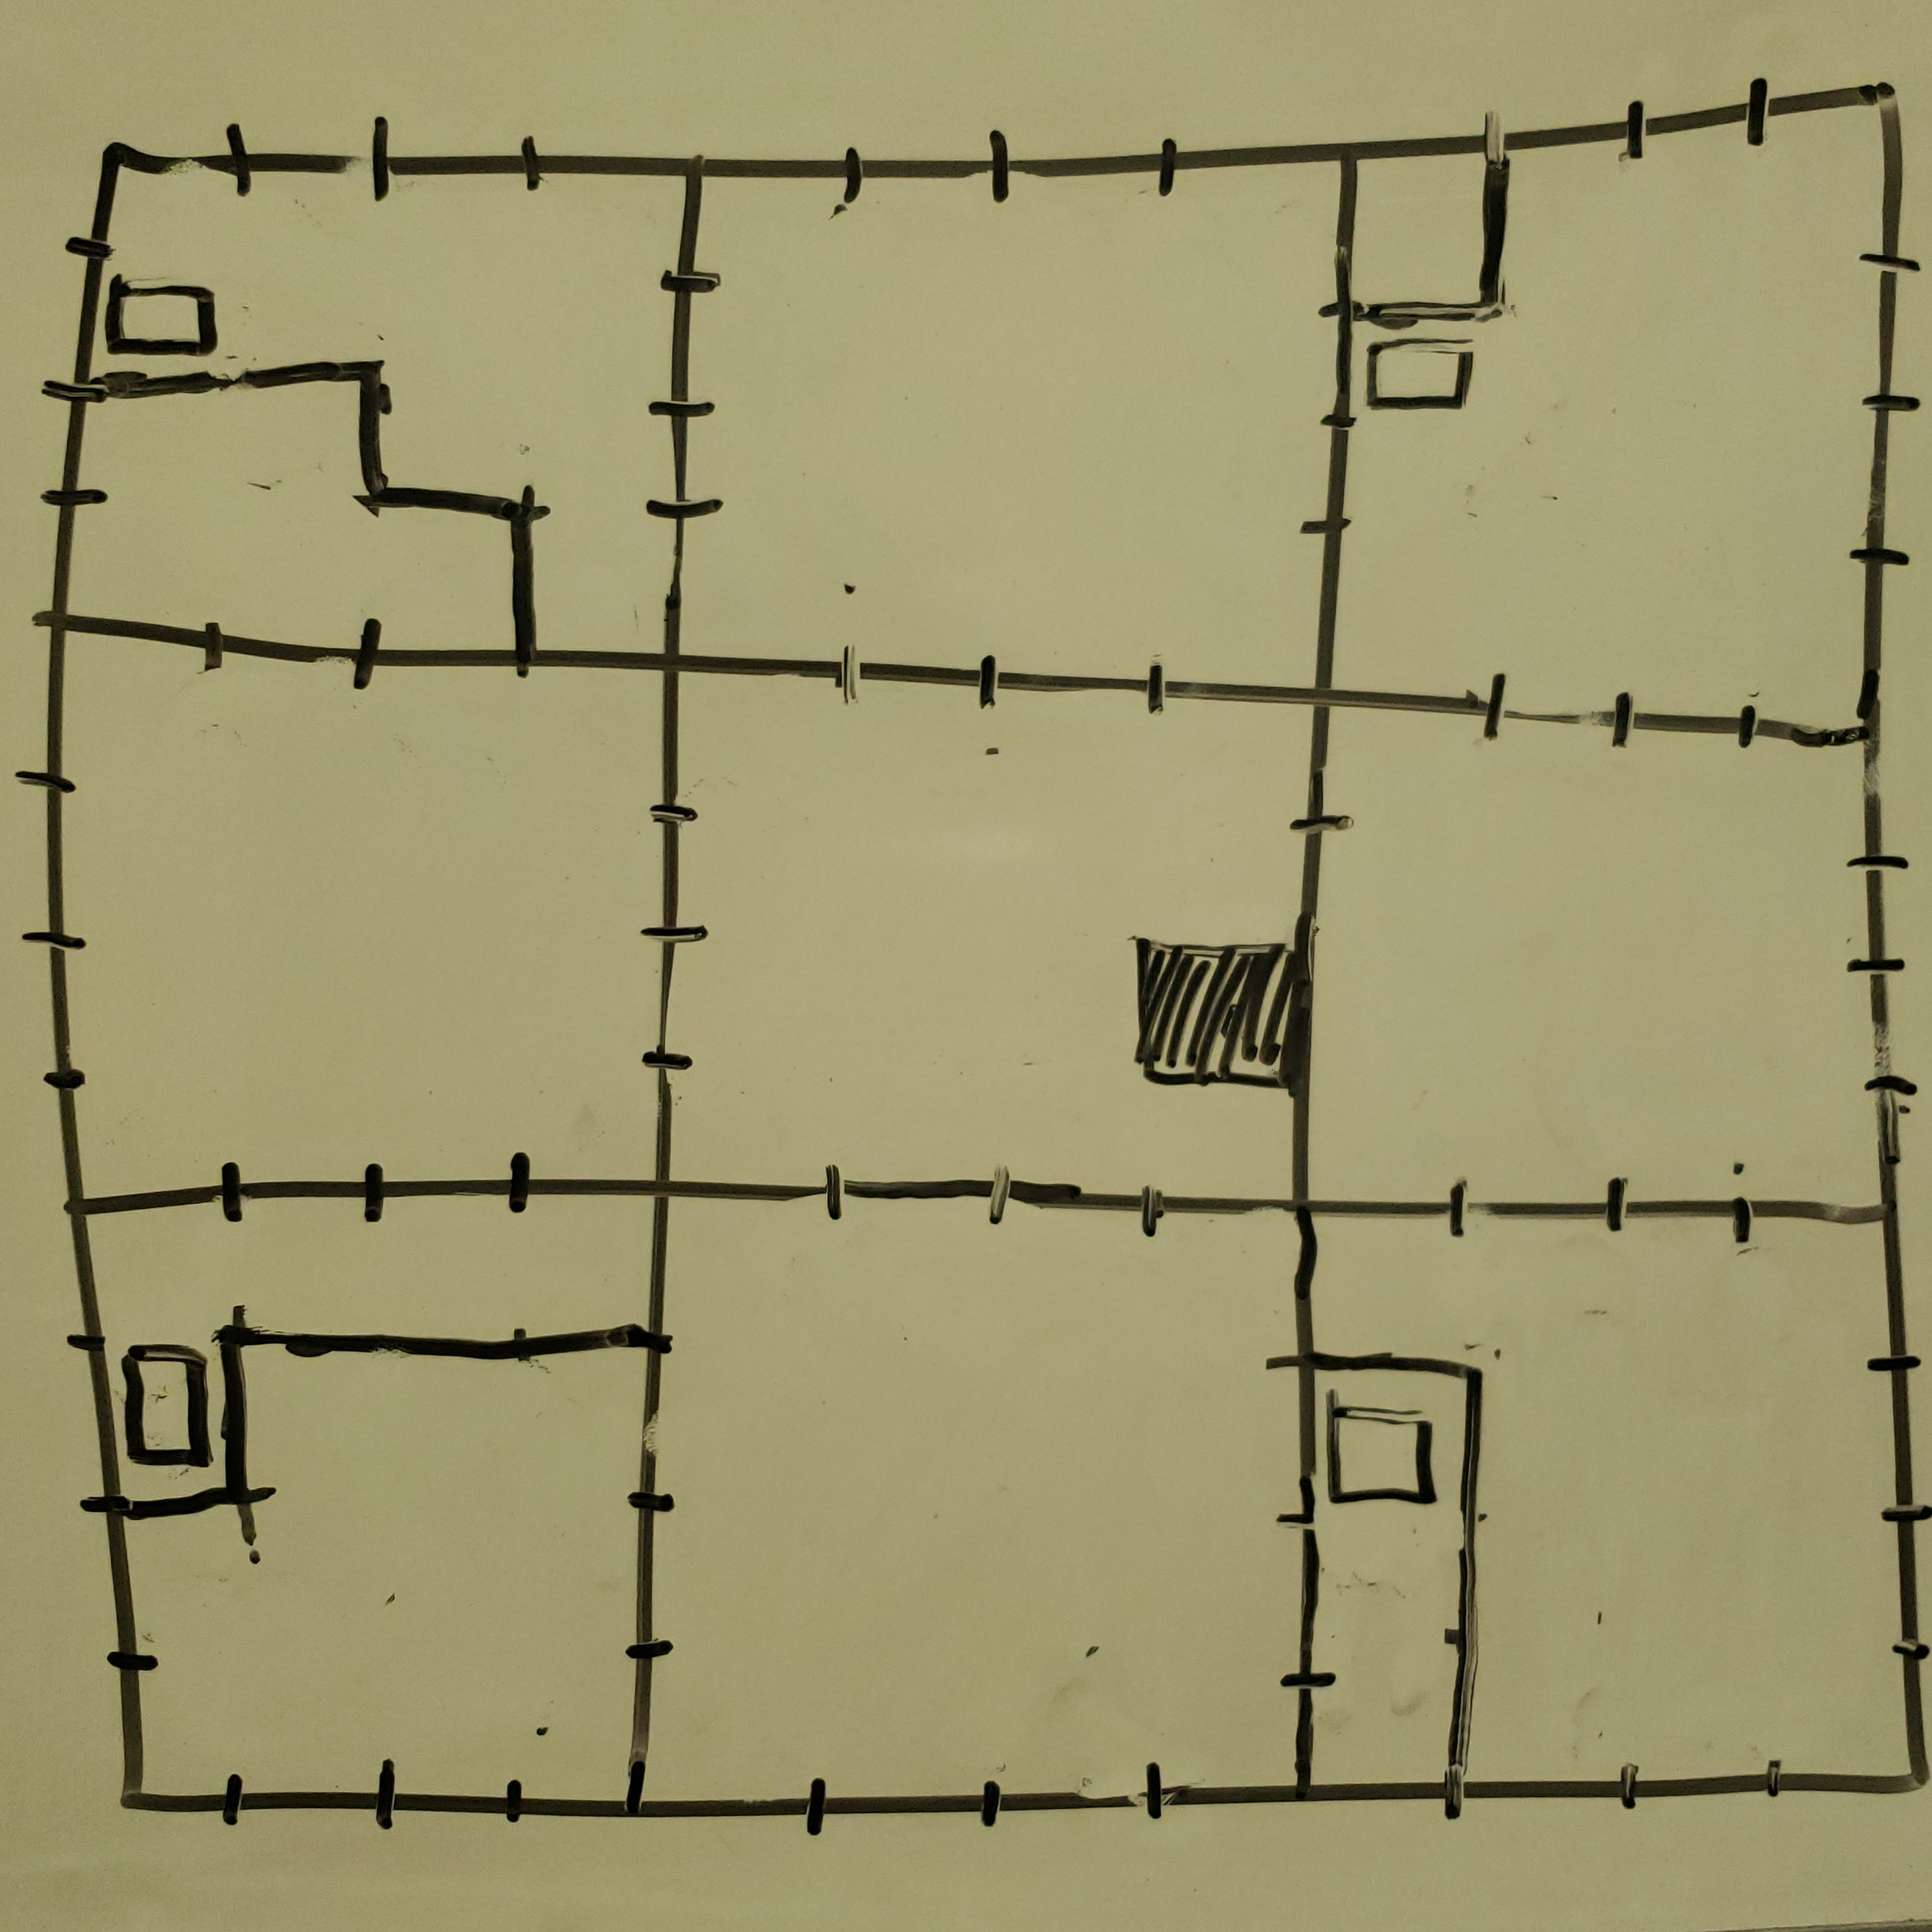
\includegraphics[width=0.5\linewidth]{grid.jpg}
\end{center}
Shaded pixel: camera \\
Lines: region boundaries \\
Inlined pixels: edge cases (given to clockwise region in this case)
\end{document}
